\section{Critical Synthesis} \label{criticalsynthesis}

\subsection{Results}
The authors suggest that investor sentiment, in general, negatively influences stock returns. There are many drivers of this phenomena, however, one of the most argued is that over-optimistic behaviour of the market players during high sentiment periods leads to lower stock market returns later. 

\paragraph{Geographical Location}
Research results differ among countries. Some countries do not exhibit any relationship between sentiment and returns, whereas others possess strong negative relationships (Schmeling 2009). Examples for countries with existing relationships are Belgium, Germany, Japan and Italy at 1\% confidence level and France, Norway, Sweden, Switzerland and US at 5\%. Moreover, he concludes, that collectivistic countries and countries with high uncertainty avoidance show larger effects of sentiment on returns than individualistic countries. Schmeling (2009) argues that one cannot transfer evidence from the US to other markets all over the world. Most of the research papers focus on the US market, as there are available various measures of investor sentiment (e.g. AAII, II). 

\paragraph{Type of Firm} Regarding the nature of the firms analysed, Smales (2017) confirms that indeed, small, hard-to-value firms are influenced more by sentiment. This is also confirmed by Schmeling (2009) on an international level, where small stocks exhibit lower returns as the sentiment grows in 1, 6 and 12 months’ periods at 1\%. Contrary to this finding, Brown and Cliff (2002) find that the strongest relationship lies between measures on institutional sentiment and large stocks. Furthermore, Fisher and Statman (2000) find that larger stocks are more influenced by the investor sentiment than small stocks. This incongruity might be assigned to different sentiment measures. Brown and Cliff (2002) and Fisher and Statman (2000) use AAII for the small stocks and Merrill Lynch data for large stocks whereas Smales (2017) uses VIX - implied volatility index – so-called "measure of fear". AAII, measures where investors think the market will be in 6 months and according to Smales (2017) is not a good predictor of the short term market, which is studied by Fisher and Statman (2000).
\par
On the international level, Schmeling (2009) confirms that small stocks are more negatively influenced by the investor sentiment than larger stocks. 
\par
Overall, the research shows that small stocks are more influenced by investor sentiment as the information to evaluate the fundamentals of small stocks is missing and investors tend to rely on an advice of semi-professional investor newsletters or make less informed decisions.

\paragraph{Recession vs Expansion} The results differ for economies in different states. Chung et al. (2012) confirmed this notion that the predictive power of investor sentiment is influenced by the economic changes. Secondly, they find that during expansion, investor sentiment has higher predictive power compared to recession. High sentiment yields lower returns for small, hard-to-value stocks and stocks which do not pay dividends. In contrary, Smales (2017) argues that changes in VIX (investor sentiment proxy) affect the stock prices more in times of recession. During expansion, there is no significant influence. He finds that fear, represented by VIX, is a better predictor of stock returns which confirms the behavioural assumptions indicated before.

\paragraph{Short-term vs Long-term} In Schmeling (2009) we see that as time passes from 1 month to 24 months, the significance and magnitude of the relationship between sentiment and stock returns weakens (from -0.42 at 5\% significance, to -0.20 at 10\% significance). Fisher and Statman (2007) confirm that 1 month lag in stock returns is significantly influenced by the investor sentiment for S\&P 500. Brown and Cliff (2004) confirm that 1 month results are significant and positive (professional sentiment → large stocks) and weekly results are not significant. Thus, determining the appropriate time lag is essential in a panel study as this will influence the results.

\paragraph{Individual vs Institutional}
According to Fisher and Statman (2000) institutional sentiment seems to play a larger role in influencing stock market returns. There is a decrease of 0.24\% in returns for each 1\% increase in institutional sentiment, compared to a 0.10\% decrease in returns for 1\% increase in individual sentiment. Furthermore, institutional sentiment seems not to be affected by stock prices as the institutions are more rational in their opinions. However, according to Brown and Cliff (2004) professional sentiment increases the stock returns in a 1 week period.
\par
Per Brown and Cliff (2002) the sentiments share many aspects; however, they only correlate with 0.43. Additional studies support the idea that the sentiments differ and have different effect on the stock returns. Brown and Cliff (2002) find that whereas institutional sentiment influences large cap stocks, the individual does not. Moreover, small cap stocks are not influenced by either sentiment. The influence of institutional sentiment and the individual sentiment between each other is also explored. It concludes that even though individual investors are influenced by the institutional sentiment, the relationship does not hold backwards. Institutional sentiment is free from the influence of individual sentiment. It seems that the institutional investors are more rational and some evidence shows that high sentiment increases the stock returns. In contrast, the sentiment of individual investors, who mainly receive information from newsletters, is an indicator of negative stock returns.

\subsubsection{Effect Sizes}
When comparing effect sizes across studies, it is important to take into consideration the specific types of returns on which the study was performed. The result of an analysis made on a specific sample cannot be generalised to the whole population or domain unless we have the certainty that the sample itself is representative enough and the results are generalizable, fact given by the research strategy employed. Thus, the following analysis groups the researches on stock analysed and sentiment used.
\par
Fisher \& Statman (2000) perform their study on the S\&P 500 index, apply a time lag of 1 month, and get an effect size of -0.1\% for individual investors and -0.24\% for Wall Street strategists. This means that if sentiment of individual investors increases by 1\%, stock returns a month later are down 0.1\%, and down 0.24\% if the Wall Street strategist sentiment increases by 1\%. This implies a stronger relationship for investors on Wall Street, making their returns more sensitive to investor sentiment. Smales (2017) performs a similar test on S\&P 500 using the implied volatility of index VIX, as proxy for investor sentiment. His results show that a 1\% increase in sentiment leads to 0.86\% decrease in the ensuing returns for the following month. Contrary to these results, Brown and Cliff (2002) find that in a timespan of one week, the S\&P 500 index shows an increase of 0.026\% if the sentiment of professionals increases by 1\%. However, this does not hold for the 6-8 deciles of NYSE/AMEX/NASDAQ, for which a rise in sentiment leads to decrease of 0.58\% in the time frame of 1 month. Although their test for lags of 2 months does not produce any significant results, combining both time lags gives another significant outcome, with regression coefficient of -0.012\%. Such coefficient suggests that the effect of investor sentiment is stronger within 1 month, and it is reduced if a longer time frame is considered.
\par
Baker and Wurgler (2007) take a more general approach and analyse market returns on common stocks from the CRSP database, also lagged by 1 month. For the independent variable, they compute their own index based on 6 variables which act as proxies in determining the value of investor sentiment. Splitting the stock returns into equal-weighted and value-weighted market returns helps in comparing their results for similarities and differences. The effect sizes of their analysis show that investor sentiment above one standard deviation from the historical average has a higher impact on the equal-weighted market index returns (-0.41\%), while it is lower for the value-weighted ones (-0.34\%). Using the same sentiment index, Dergiades (2012) searches for non-linear causality between sentiment and 1 month lagged US stock prices’ index from 2005. The two tests employed by them, Hiemstra and Jones (1994) and Diks and Panchenko (2006), provide a rejection of the null hypothesis on 3 out of the 5 lags, pointing to the existence of a non-linear causal relationship.

\subsubsection{Managerial Relevance of the Effect Sizes}
The relevant parameter for managers in these studies is the effect size as a regression coefficient, which provides the magnitude of the effect of sentiment over stock returns. These results inform the investors of the potential decrease that may follow a period of high investor sentiment, or the expected increase in returns after periods of low sentiment. The current research does not assess the question of what is the relevant effect size necessary to employ profitable strategies based on analysis of investor sentiment. However, it is essential that the benefits of the strategy are larger than the trading costs which connect to its execution.

\subsubsection{Degree of Support of the Hypothesis}
There is a high degree of similarity between the hypotheses used in the discussed articles and the main hypothesis of our research. However, there is no clear definition on how to compute sentiment, and the variety of stocks traded worldwide makes it  difficult to conduct a general research. Most of the studies are focused on specific elements of the studied domain, aiming to find the effect of sentiment over a certain subgroup (S\&P 500, small/large cap stocks, growth stocks). Also, a wide range of options to compute investor sentiment shows there is no "right" way of measuring the sentiment, and it is the choice of the researcher to employ any direct measures or proxies that give a fair indication of the sentiment. The main takeaway from most studies is the negative relationship between investor sentiment and subsequent stock returns for parts of their employed sentiment measures and stocks. Thus, it can be concluded that current literature presents strong support for the hypothesis that sentiment has influence over the stock returns.

\subsubsection{Overview of Selected Articles}

\begin{longtable}{@{}llll@{}}
\caption{Article Summary}\\
\label{article-overview}\\
\toprule
\textbf{Article} & \textbf{\begin{tabular}[c]{@{}l@{}}Study \\ (sentiment → returns)\end{tabular}} & \textbf{Effect size} & \textbf{\begin{tabular}[c]{@{}l@{}}Precision \\ (confidence interval)\end{tabular}} \\ \midrule
\multirow{3}{*}{\begin{tabular}[c]{@{}l@{}}Investor\\ sentiment and \\ stock returns, \\ Fisher and \\ Statman (2000)\end{tabular}} & \begin{tabular}[c]{@{}l@{}}Individual investors’ \\ sentiment → S\&P 500 \\ (1 month)\end{tabular} & \begin{tabular}[c]{@{}l@{}}1\% increase in \\ sentiment level → \\ 0.1\% decrease in S\&P \\ return next month\end{tabular} & \begin{tabular}[c]{@{}l@{}}Significant, 1\% level\\ T-statistic: -2.76\\ Adj. $R^2$ = 0.05 \\ Durbin-Watson = 1.91\end{tabular} \\ \cmidrule(l){2-4} 
 & \begin{tabular}[c]{@{}l@{}}Wall Street strategists’ \\ sentiment → S\&P 500 \\ (1 month)\end{tabular} & \begin{tabular}[c]{@{}l@{}}1\% increase in \\ sentiment level → \\ 0.24\% decrease in S\&P \\ return next month\end{tabular} & \begin{tabular}[c]{@{}l@{}}Significant (no level)\\ T-statistic: -2.41\\ Adj. $R^2$ = 0.03\\ Durbin-Watson = 2.14\end{tabular} \\ \cmidrule(l){2-4} 
 & \begin{tabular}[c]{@{}l@{}}Individual, Wall Street \\ investors and newsletter \\ writers aggregated \\ sentiment → S\&P 500  \\ (1 month) - correlation\end{tabular} & \begin{tabular}[c]{@{}l@{}}$R^2$ = 0.08 Sentiment \\ explains 8\% of the \\ variation in \\ S\&P 500 returns\end{tabular} & \begin{tabular}[c]{@{}l@{}}Significant, 1\% level\\ Adj. $R^2$ = 0.08\\ Durbin-Watson = 1.98\end{tabular} \\ \midrule
\multirow{4}{*}{\begin{tabular}[c]{@{}l@{}}The importance\\  of fear: \\ investor \\ sentiment and \\ stock market \\ returns, \\ Smales (2017)\end{tabular}} & \begin{tabular}[c]{@{}l@{}}VIX → S\&P 500\\ (1 month)\end{tabular} & \begin{tabular}[c]{@{}l@{}}1\% increase in \\ sentiment → \\ 0.86 \% decrease \\ in S\&P 500 return\end{tabular} & \begin{tabular}[c]{@{}l@{}}Significant: 1 \% level\\ AIC = 3.939\\ Durbin-Watson = 2.730\\ Wald F-stat = 146\end{tabular} \\ \cmidrule(l){2-4} 
 & \begin{tabular}[c]{@{}l@{}}VIX → large cap stocks\\ (1 month)\end{tabular} & \begin{tabular}[c]{@{}l@{}}1\% increase in \\ sentiment → \\ 0.014\% increase \\ in return\end{tabular} & \begin{tabular}[c]{@{}l@{}}Not significant: 10\% level\\ AIC = 5.704\\ Durbin-Watson = 2.004\\ Wald F-stat = 5.965\end{tabular} \\ \cmidrule(l){2-4} 
 & \begin{tabular}[c]{@{}l@{}}AAII → small cap stocks \\ (1 month)\end{tabular} & \begin{tabular}[c]{@{}l@{}}1\% increase in \\ sentiment → \\ 0.039 \% increase \\ in return\end{tabular} & \begin{tabular}[c]{@{}l@{}}Not significant: 10\% level\\ AIC = 6.438\\ Durbin-Watson = 2.020\\ Wald F-stat = 1.742\end{tabular} \\ \cmidrule(l){2-4} 
 & \begin{tabular}[c]{@{}l@{}}VIX → growth stocks \\ (1 month)\end{tabular} & \begin{tabular}[c]{@{}l@{}}1\% increase in \\ sentiment → 0.03 \% \\ decrease in return\end{tabular} & \begin{tabular}[c]{@{}l@{}}Not significant: 10\% level \\ AIC = 5.804\\ Durbin-Watson = 2.020\\ Wald F-stat = 3.866\end{tabular} \\ \midrule

\multirow{12}{*}{\begin{tabular}[c]{@{}l@{}}Investor \\ sentiment and\\ the near-term\\ stock market, \\ Brown and \\ Cliff (2002)\end{tabular}} & \begin{tabular}[c]{@{}l@{}}Kalman filter - \\sentiment of \\ professionals → \\ S\&P 500 (1 week)\end{tabular} & \begin{tabular}[c]{@{}l@{}}Combined lags\\ 1\% increase in \\ sentiment → 0.03\% \\ increase in return \end{tabular} & \begin{tabular}[c]{@{}l@{}}Significant:\\ 5\% level\end{tabular} \\  \cmidrule(l){2-4} 
 & \begin{tabular}[c]{@{}l@{}}Kalman filter \\(AAII, II) → \\ Russell 2000 Index\\ (1 week)\end{tabular} & \begin{tabular}[c]{@{}l@{}}Combined lags\\ 1\% increase in \\ sentiment → \\ 0.08\% decrease \\in return \end{tabular} & Not significant: 10\% level \\ \cmidrule(l){2-4} 
 
 & \multirow{3}{*}{\begin{tabular}[c]{@{}l@{}}Kalman filter \\(AAII, II) → \\ Largest quintile\\ NYSE/AMEX/\\NASDAQ\end{tabular}} 
 
 & \begin{tabular}[c]{@{}l@{}}Lag 1 month\\ 1\% increase in \\ sentiment → \\ 0.26\% increase\\ in return \end{tabular} & Not significant: 10\% level \\ \cmidrule(l){3-4} 

&  & \begin{tabular}[c]{@{}l@{}}Lag 2 months\\ 1\% increase in \\ sentiment → \\ 0.11\% decrease \\in return\end{tabular} & Not significant: 10\% level \\ \cmidrule(l){3-4} 

&  & \begin{tabular}[c]{@{}l@{}}Combined lags\\ 1\% increase in \\ sentiment → \\  0.8\% decrease \\in return\end{tabular} & Not significant: 10\% level \\ \cmidrule(l){2-4} 
 
 & \multirow{3}{*}{\begin{tabular}[c]{@{}l@{}}Kalman filter \\(AAII, II) → \\ 6-8 deciles\\ NYSE/AMEX/NASDAQ\end{tabular}} 
 
 & \begin{tabular}[c]{@{}l@{}}Lag 1 month\\ 1\% increase in \\ sentiment → \\ 0.58\% decrease \\in return \end{tabular} & Significant: 10\% level \\ \cmidrule(l){3-4} 
 &  & \begin{tabular}[c]{@{}l@{}}Lag 2 months\\ 1\% increase in \\ sentiment → \\ 0.003\% decrease\\ in return \end{tabular} & Not significant: 10\% level \\ \cmidrule(l){3-4} 
 &  & \begin{tabular}[c]{@{}l@{}}Combined lags \\ 1\% increase in \\ sentiment → \\ 0.01\% decrease \\in return \end{tabular} & Significant: 5\% level \\ 
 \midrule
\multirow{2}{*}{\begin{tabular}[c]{@{}l@{}}Investor \\ Sentiment in \\ the Stock \\ Market, \\ Baker and \\ Wurgler (2007)\end{tabular}} & \begin{tabular}[c]{@{}l@{}}Sentiment index from \\ 6 proxies → \\equal-weighted market \\index returns on \\ common stocks \\from CRSP database \\(1 month)\end{tabular} & \begin{tabular}[c]{@{}l@{}}Sentiment levels above \\ one standard deviation \\ from historical \\average → \\ -0.41\% stock returns.\end{tabular} & Significant: 10\% level \\ \cmidrule(l){2-4} 
 & \begin{tabular}[c]{@{}l@{}}Sentiment index from \\ 6 proxies → \\value-weighted \\ returns on common  stocks \\ from CRSP database\\ (1 month)\end{tabular} & \begin{tabular}[c]{@{}l@{}}Sentiment levels above \\ one standard deviation \\ from historical \\average → \\ -0.34\% stock returns.\end{tabular} & \begin{tabular}[c]{@{}l@{}}Significant:\\ 10\% level\end{tabular} \\ 
\midrule

\begin{tabular}[c]{@{}l@{}}Do investors’ \\ sentiment \\ dynamics \\ affect stock\\ returns? \\ Evidence from \\ the US economy, \\ Dergiades (2012)\end{tabular} & \begin{tabular}[c]{@{}l@{}}US investor sentiment \\ computed by Baker and \\ Wurgler (2007) → \\ US stock prices’ \\ index from 2005 \\ (1 month)\end{tabular} & \begin{tabular}[c]{@{}l@{}}Nonlinear causality \\tests by Hiemstra \& \\Jones  (1994) and Diks\\ \& Panchenko (2006)\\ show a rejection of null \\ hypothesis on 3 out \\ of 5 lags, implying a \\ nonlinear causal \\ relationship of \\ sentiment over \\ stock returns\end{tabular} & \begin{tabular}[c]{@{}l@{}}The results are significant \\ at the 5\% level for the \\ 1st and 5th lag, and at 10\% \\ for the 4th lag\end{tabular} \\ \midrule

\multirow{12}{*}{\begin{tabular}[c]{@{}l@{}}Investor \\ sentiment \\and stock \\returns: some \\international \\evidence \\ Schmeling (2009)\end{tabular}} 

& \begin{tabular}[c]{@{}l@{}}Consumer confidence → \\ CRSP aggregate \\stock market\\ (1 month)\end{tabular} & \begin{tabular}[c]{@{}l@{}} 1\% increase in \\ sentiment → 0.31\% \\ decrease in returns \end{tabular} & \begin{tabular}[c]{@{}l@{}}Significant: 5\% level\\Adj. $R^2$ = 0.06\end{tabular} \\ \cmidrule(l){2-4}

& \begin{tabular}[c]{@{}l@{}}Consumer confidence → \\ CRSP aggregate \\stock market\\ (6 month)\end{tabular} & \begin{tabular}[c]{@{}l@{}} 1\% increase in \\ sentiment → 0.31\% \\ decrease in returns \end{tabular} & \begin{tabular}[c]{@{}l@{}}Significant: 5\% level\\Adj. $R^2$ = 0.06\end{tabular} \\ \cmidrule(l){2-4}

& \begin{tabular}[c]{@{}l@{}}Consumer confidence → \\ CRSP aggregate \\stock market\\ (12 month)\end{tabular} & \begin{tabular}[c]{@{}l@{}} 1\% increase in \\ sentiment → 0.26\% \\ decrease in returns \end{tabular} & \begin{tabular}[c]{@{}l@{}}Significant: 5\% level\\Adj. $R^2$ = 0.11\end{tabular} \\ \cmidrule(l){2-4}

& \begin{tabular}[c]{@{}l@{}}Consumer confidence → \\ CRSP aggregate \\stock market\\ (24 month)\end{tabular} & \begin{tabular}[c]{@{}l@{}} 1\% increase in \\ sentiment → 0.20\% \\ decrease in returns \end{tabular} & \begin{tabular}[c]{@{}l@{}}Significant: 5\% level\\Adj. $R^2$ = 0.19\end{tabular} 

\\\midrule 
 
\multirow{12}{*}{\begin{tabular}[c]{@{}l@{}}When does \\ investor sentiment\\ predict stock \\returns? \\ Chung et al. \\(2012)\end{tabular}} 

& \begin{tabular}[c]{@{}l@{}}Baker and Wurgler \\ sentiment → US stock \\market returns\end{tabular} & \begin{tabular}[c]{@{}l@{}} 1\% increase in \\ sentiment → 0.71\% \\ increase in returns \end{tabular} & \begin{tabular}[c]{@{}l@{}}Significant: 1\% level\end{tabular} \\ \cmidrule(l){2-4}
 
& \begin{tabular}[c]{@{}l@{}}Baker and Wurgler \\ sentiment → US stock \\market returns\\(Recession)\end{tabular} & \begin{tabular}[c]{@{}l@{}} 1\% increase in \\ sentiment → 0.06\% \\ decrease in returns \end{tabular} & \begin{tabular}[c]{@{}l@{}}Not significant\\ at 10\% level\end{tabular} \\ \cmidrule(l){2-4}

& \begin{tabular}[c]{@{}l@{}}Baker and Wurgler \\ sentiment → US stock \\market returns\\(Expansion)\end{tabular} & \begin{tabular}[c]{@{}l@{}} 1\% increase in \\ sentiment → 1.03\% \\ increase in returns \end{tabular} & \begin{tabular}[c]{@{}l@{}}Significant: 1\% level\end{tabular} 

\\\midrule 

\multirow{12}{*}{\begin{tabular}[c]{@{}l@{}}Do measures \\ of investor \\sentiment predict \\returns?\\ Neal and \\Wheatley (1998)\end{tabular}} 

& \begin{tabular}[c]{@{}l@{}}Discount on \\closed ended funds → \\ Stock returns \\on NYSE-AMEX\\ (1 month)\end{tabular} & \begin{tabular}[c]{@{}l@{}} 1 standard deviation\\ increase in discount\\→ 0.36\% increase in \\returns\end{tabular} & \begin{tabular}[c]{@{}l@{}}Significant: 5\% level\end{tabular} \\ \cmidrule(l){2-4}

& \begin{tabular}[c]{@{}l@{}}Discount on \\closed ended funds → \\ Stock returns \\on NYSE-AMEX\\ (4 month)\end{tabular} & \begin{tabular}[c]{@{}l@{}} 1 standard deviation\\ increase in discount\\→ 0.52\% increase in \\returns\end{tabular} & \begin{tabular}[c]{@{}l@{}}Significant: 10\% level\end{tabular} \\ \cmidrule(l){2-4}

& \begin{tabular}[c]{@{}l@{}}Discount on \\closed ended funds → \\ Stock returns \\on NYSE-AMEX\\ (12 month)\end{tabular} & \begin{tabular}[c]{@{}l@{}} 1 standard deviation\\ increase in discount\\→ 0.91\% increase in \\returns\end{tabular} & \begin{tabular}[c]{@{}l@{}}Significant: 5\% level\end{tabular}

\\\bottomrule

\end{longtable}

\subsection{Quantitative Review}
As summarized in Critical Evaluation (Section~\ref{critical-evaluation}) and the articles overview in Table~\ref{article-overview}, past studies differ considerably in their research methodologies. Moreover, there is a wide range of specific time lags and sentiment measure for which useful results were found. Figure~\ref{fig:figure20} shows the range of selected effect sizes and how they compare to effect sizes found in comparable studies.

\begin{figure}[ht]
\centering
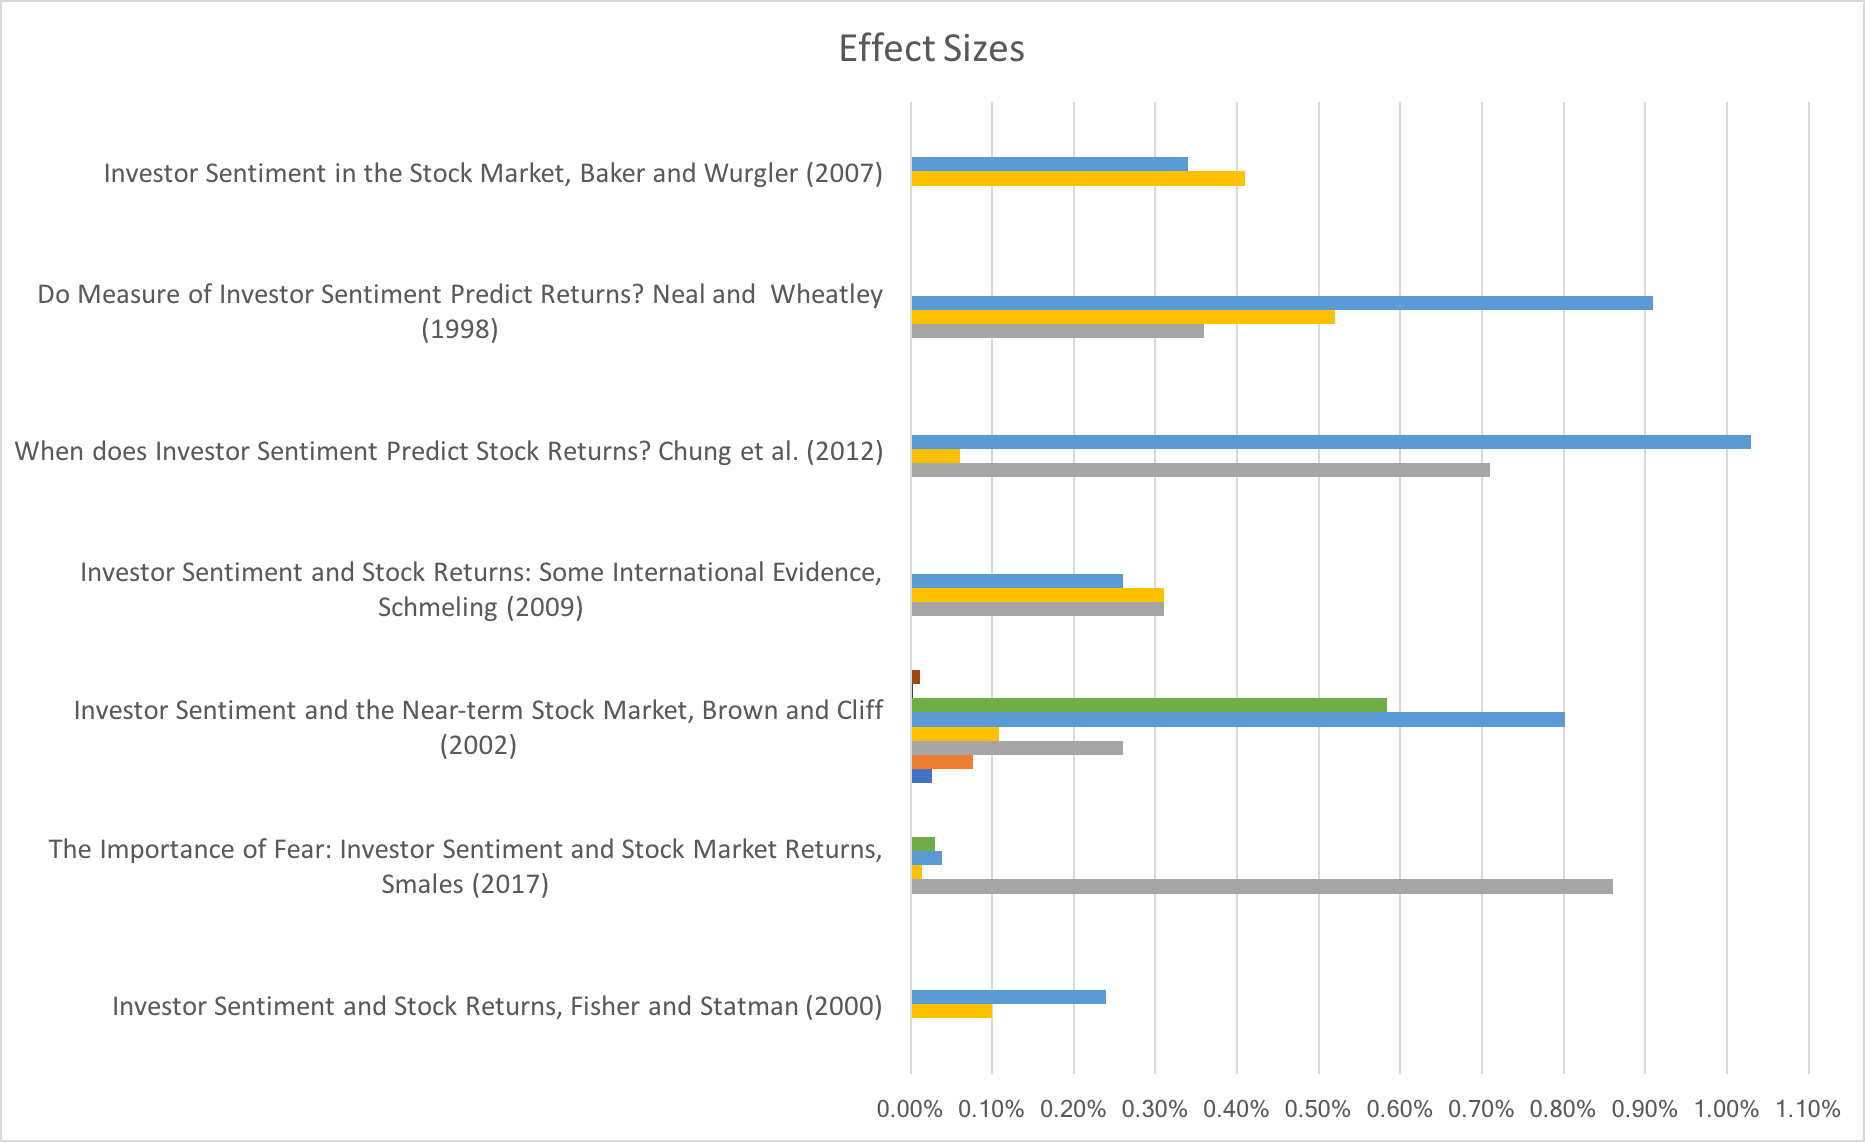
\includegraphics[width=1\textwidth]{figures/effect-size.png}
\caption{\label{fig:figure20}Selected Range of Effect Sizes of Past Studies. In Baker and Wurgler (2007) and Neal \& Wheatley (1998) the effect size is the change in returns if sentiment is one standard deviation above normal. For the remaining studies the effect size is the percentage change in return after one percent change in sentiment.}
\end{figure}

The data of Figure~\ref{fig:figure20} includes results from a variety of time lags from 1 to 6 months, as well as different sentiment measures, such as AAII or VIX. The effect size itself is: the percentage change in return if sentiment deviates by one standard deviation from historical average for Baker and Wurgler (2007) and Neal and Wheatley (1998); or the percentage change in stock returns after one percent change in sentiment level for the remaining studies. All studies found that investor sentiment and stock returns are negatively related. To mirror this finding in Figure~\ref{fig:figure20}, we inverted some of the effect sizes to receive a concise overview focusing on the strength of the relationship. The inversion was necessary because some studies, particularly Smales (2017), use a fear indicator instead of positive sentiment. Remarkably, no effect size approaches 1\%, except one finding by Chung et al. (2012). The change in stock returns is almost always smaller than the change in sentiment. Apart from that, the range of effect sizes is widespread between 0\% and 0.9\%. Conclusively, while there is agreement on the existence of a negative relationship, the effect size varies widely. This is caused by different measurements, methodologies and markets and stocks researched applied by the researchers. 